\documentclass{article}
\usepackage{amsmath}
\usepackage{amssymb}
\usepackage{graphicx}
\usepackage{hyperref}
\usepackage[version=4]{mhchem}


\begin{document}
\section*{Problem}
In \(\triangle A B C, A B=A C\). \(E\) is the midpoint of \(A B\). Extend \(A B\) to \(D\) such that \(B D=B A\). Prove: \(C D=2 C E\).\\
\centering
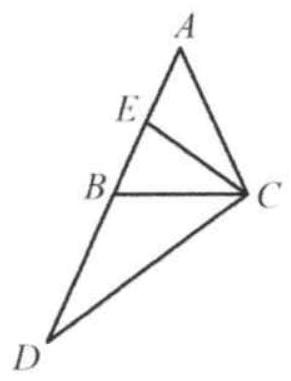
\includegraphics[width=\textwidth]{images/027(1).jpg}

\section*{Solution}
Method 1:\\
Extend \(C E\) to \(F\) such that \(C E=E F\). Since \(A E=E B\) and \(\angle 1=\angle 2, \triangle A E C \cong \triangle B E F\).\\
Thus, \(\angle 3=\angle F, \angle 4=\angle A, B F=A C\). Since \(A B=A C=B D\), therefore \(B F=B D\). \(\angle D B C=\angle A+\angle A C B=\angle A+\angle A B C\) or \(\angle F B C=\angle 4+\) \(\angle A B C=\angle A+\angle A B C\).

Thus, \(\angle D B C=\angle F B C\). Since \(B C=B C, \triangle F B C \cong \triangle D B C\).\\
Therefore \(C F=C D\).\\
Since \(C E=E F=1 / 2 C F=1 / 2 C D, C D=2 C E\).\\
\centering
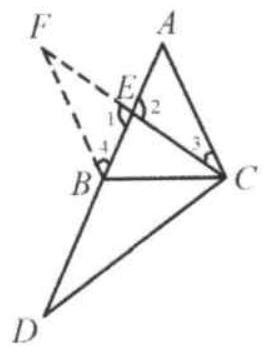
\includegraphics[width=\textwidth]{images/030.jpg}

Method 2:\\
Extend \(C E\) to \(F\) such that \(C E=E F\). Since \(A E=E B\) and \(\angle 1=\angle 2, \triangle A E F \cong \triangle B E C\).\\
Thus, \(\angle 3=\angle F, \angle 4=\angle C B E, A F=B C\). Since \(A B=A C=B D, A C=B D\).\\
\(\angle D B C=\angle C A B+\angle A C B=\angle C A B+\angle A B C\)\\
\(\angle C A F=\angle C A B+\angle 4=\angle C A B+\angle A B C\).\\
Thus, \(\angle D B C=\angle C A F\). Since \(A F=B C, A C=B D\), so \(\triangle F A C\) \(\cong \triangle C B D\).\\
\centering
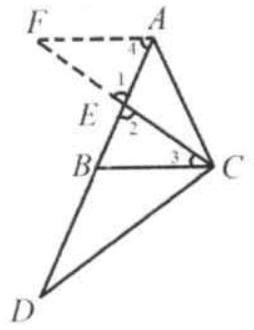
\includegraphics[width=\textwidth]{images/030(2).jpg}

Therefore \(C F=C D\).\\
Since \(C E=E F=1 / 2 C F=1 / 2 C D, C D=2 C E\).

\end{document}
